
\begin{figure*}[t]
\centering
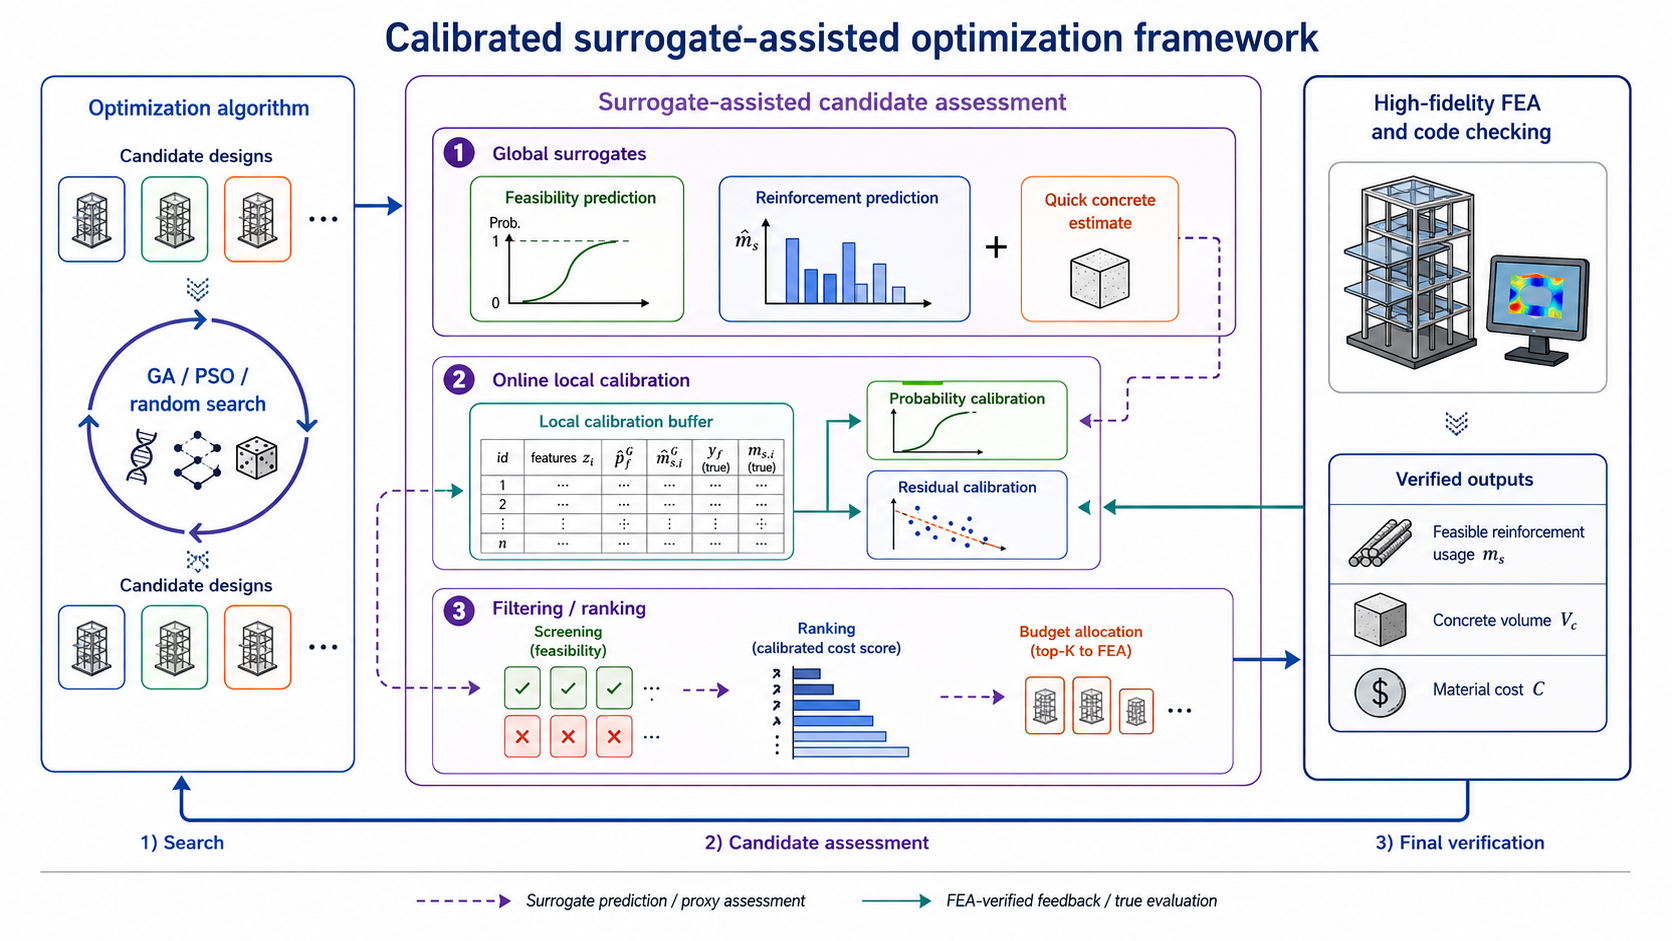
\includegraphics[width=\textwidth]{calibrated_optimization_framework.png}
\caption{Calibrated surrogate-assisted optimization framework.}
\label{fig:calibrated_optimization_framework}
\end{figure*}

\section{Calibrated Surrogate-Assisted Optimization Framework}
\label{sec:optimization_framework}

This section further describes how these models are embedded into an optimization process. 

\subsection{Overall Framework}
\label{subsec:overall_framework}

The overall framework is illustrated in Fig.~\ref{fig:calibrated_optimization_framework}. For a fixed shear wall layout $L$ and design condition $c$, the optimization task is to search the design space $\mathcal{X}$ for section and material parameters that minimize the material cost while satisfying all structural checks. At iteration $t$, the optimizer $\mathcal{O}$ generates a batch of candidate designs:
\begin{equation}
\mathcal{B}_t=
\left\{
x_{t,1},x_{t,2},\ldots,x_{t,N_b}
\right\},
\label{eq:candidate_batch}
\end{equation}
where $N_b$ is the batch size.

For each candidate $x_{t,i}$, the corresponding input representation is constructed as a structured tuple:
\begin{equation}
z_{t,i}=\left(G,q,d_{t,i}\right),
\label{eq:candidate_input_framework}
\end{equation}
where $G$ is the room-level layout graph, $q$ is the vector of global layout statistics, and $d_{t,i}$ is the design-parameter vector formed by $x_{t,i}$ and the design condition $c$. This notation indicates that graph features, global layout statistics, and design parameters are passed to the surrogate model as separate input components and fused inside the model. Since the layout and design condition remain fixed in a single optimization task, $G$ and $q$ are constant, while $d_{t,i}$ varies among candidates.

The global surrogate models first provide feasibility and reinforcement predictions for all candidates:
\begin{equation}
\hat{p}_{f,t,i}^{G}=SM_f(z_{t,i}),
\label{eq:global_feasibility_framework}
\end{equation}
\begin{equation}
\hat{m}_{s,t,i}^{G}=SM_s(z_{t,i}).
\label{eq:global_steel_framework}
\end{equation}
If the local calibration set $\mathcal{D}_{t}^{loc}$ contains enough verified samples to fit the calibration models, the global predictions are corrected by the online calibration module:
\begin{equation}
\hat{p}_{f,t,i}^{C}=\mathcal{C}_{f,t}(\hat{p}_{f,t,i}^{G}),
\label{eq:calibrated_feasibility_framework}
\end{equation}
\begin{equation}
\hat{m}_{s,t,i}^{C}=\mathcal{C}_{s,t}(z_{t,i},\hat{m}_{s,t,i}^{G}),
\label{eq:calibrated_steel_framework}
\end{equation}
where $\mathcal{C}_{f,t}$ and $\mathcal{C}_{s,t}$ denote the feasibility probability calibration model and the reinforcement residual calibration model at iteration $t$, respectively.

The calibrated predictions are then used for candidate screening and priority ranking. The candidate subset selected for true evaluation is denoted by $\mathcal{S}_t\subseteq \mathcal{B}_t$. For each candidate in $\mathcal{S}_t$, the true evaluator produces FEA-verified results:
\begin{equation}
\mathcal{E}(L,c,x_{t,i})
\rightarrow
(y_{f,t,i},m_{s,t,i},m_{c,t,i},r_{t,i}),
\quad x_{t,i}\in\mathcal{S}_t .
\label{eq:true_eval_framework}
\end{equation}
These verified results are used to update the optimizer and to expand the local calibration set.

\subsection{Candidate Screening and Priority Ranking}
\label{subsec:candidate_screening_ranking}

The surrogate-based pre-evaluation module consists of two consecutive operations, feasibility screening and priority ranking. The first operation aims to reduce unnecessary FEA calls for candidates that are very unlikely to satisfy the structural checks. The second operation prioritizes candidates that are more likely to achieve low material cost under the limited FEA budget.

Given the calibrated feasibility probability $\hat{p}_{f,t,i}^{C}$ and the screening threshold $\tau_t$, the candidates passing the feasibility screening are defined as
\begin{equation}
\mathcal{B}_{t}^{pass}
=
\left\{
x_{t,i}\in\mathcal{B}_t
\mid
\hat{p}_{f,t,i}^{C}\ge \tau_t
\right\}.
\label{eq:pass_set}
\end{equation}
The threshold $\tau_t$ follows the conservative strategy introduced in Section~\ref{subsec:online_local_calibration}. Its purpose is to avoid removing potentially feasible designs.

Because the optimizers minimize a scalar objective value, candidates that are not submitted to FEA still need a placeholder fitness for optimizer bookkeeping. These candidates, including those rejected by screening or skipped after ranking, are assigned a large rejected objective:
\begin{equation}
F^{rej}(x_{t,i}) = M_{rej},
\quad M_{rej}=1.0\times 10^{12}.
\label{eq:rejected_objective}
\end{equation}
This value is much larger than normal material-cost or penalty values, so such candidates are dominated in the minimization process and are effectively skipped by the optimizer. The rejected objective is not a verified infeasibility label and is not used for best-solution comparison or local calibration.

For a truly evaluated candidate design ${x}_{t,i}$, the scalar fitness used by the optimizer is defined as
\begin{equation}
F({x}_{t,i})
=
\begin{cases}
C({x}_{t,i}), 
& {x}_{t,i}\in\Omega_f,\\[3pt]
P_0+\lambda_v V({x}_{t,i})+\lambda_c C({x}_{t,i}),
& {x}_{t,i}\notin\Omega_f,
\end{cases}
\label{eq:true_fitness}
\end{equation}
where $C({x}_{t,i})$ is the material cost, $\Omega_f$ denotes the feasible domain, $P_0$ is a base infeasibility penalty, and $\lambda_v$ and $\lambda_c$ are the violation and cost weights for infeasible candidates. The violation measure is
\begin{equation}
\begin{aligned}
V({x}_{t,i})
={}&
\sum_{r}
\max\left(
0,
\frac{g_r({x}_{t,i})-g_r^{\lim}}{g_r^{\lim}}
\right) \\
&+
\sum_{s}
\max\left(
0,
\frac{h_s^{\lim}-h_s({x}_{t,i})}{h_s^{\lim}}
\right) \\
&+
\sum_{q} b_q({x}_{t,i}),
\end{aligned}
\label{eq:violation_score}
\end{equation}
where $g_r$ denotes upper-bound constraints, $h_s$ denotes lower-bound constraints, and $b_q\in\{0,1\}$ indicates whether a discrete code-check item fails. Therefore, infeasible candidates are primarily ranked by their degree of code violation, while feasible candidates are ranked directly by material cost.


For a candidate that is not rejected by the feasibility screener, The surrogate ranking score is then defined as
\begin{equation}
S_{t,i}^{C}
=
\hat{C}_{t,i}^{C}
+
\eta
\max(0,p_0-\hat{p}_{f,t,i}^{C}),
\label{eq:ranking_score}
\end{equation}
where $\hat{p}_{f,t,i}^{C}$ is the calibrated feasibility probability, $p_0$ is the feasibility hinge threshold, and $\eta$ is the risk-penalty coefficient.


The FEA budget at iteration $t$ is adaptive. Before any feasible design has been observed, a larger budget is used:
\begin{equation}
K_t^{pre}
=
\max
\left(
K_{\min},
\left\lceil r_{pre}|\mathcal{B}_t^{pass}|\right\rceil
\right),
\label{eq:pre_feasible_budget}
\end{equation}
where $r_{pre}=0.8$ in the experiments. The selected set is obtained by the lowest surrogate scores:
\begin{equation}
\mathcal{S}_t
=
\mathrm{TopK}
\left(
\mathcal{B}_t^{pass}, S_{t,i}^{C}, K_t^{pre}
\right).
\label{eq:pre_feasible_selection}
\end{equation}

After at least one feasible design has been found, the selection switches to a mixed strategy:
\begin{equation}
K_t
=
\max
\left(
K_{\min},
\left\lceil r|\mathcal{B}_t^{pass}|\right\rceil
\right),
\label{eq:post_feasible_budget}
\end{equation}
and
\begin{equation}
\mathcal{S}_t
=
\mathcal{S}_t^{cost}
\cup
\mathcal{S}_t^{risk}
\cup
\mathcal{S}_t^{div},
\label{eq:mixed_selection}
\end{equation}
where $\mathcal{S}_t^{cost}$ contains the candidates with the lowest surrogate cost scores, $\mathcal{S}_t^{risk}$ contains candidates with the lowest feasibility risk, and $\mathcal{S}_t^{div}$ is a randomly sampled exploration subset. In the experiments, the three quotas are set to 60\%, 25\%, and 15\% of $K_t$, respectively. If the union contains fewer than $K_t$ candidates, the remaining budget is filled by the lowest-score candidates not yet selected.



Through this two-stage mechanism, the feasibility surrogate and the reinforcement surrogate have different but complementary functions. The feasibility surrogate reduces the probability that clearly infeasible candidates consume FEA calls, whereas the reinforcement surrogate ranks the remaining candidates by material economy. Online local calibration improves both decisions by adapting the global surrogate predictions to the current layout and search region.

\subsection{Online Update with FEA-Verified Samples}
\label{subsec:online_update_framework}

After the selected candidates $\mathcal{S}_t$ are evaluated by the true evaluator, their verified results are used in two ways. First, they are used by the optimizer to update the search state. For a feasible candidate, the true material cost is calculated from the verified reinforcement and concrete quantities:
\begin{equation}
C_{t,i}
=
\pi_s m_{s,t,i}
+
\pi_c m_{c,t,i},
\quad y_{f,t,i}=1 .
\label{eq:true_cost_framework}
\end{equation}
This value is used as the true objective value for optimizer update and best-solution comparison. Infeasible candidates are handled according to the constraint-handling strategy of the optimizer.

Second, the same verified samples are added to the local calibration set:
\begin{equation}
\begin{aligned}
\mathcal{D}_{t+1}^{loc}
=
\mathcal{D}_{t}^{loc}
\cup
\bigl\{
&(z_{t,i},
\hat{p}_{f,t,i}^{G},
\hat{m}_{s,t,i}^{G},
y_{f,t,i},
m_{s,t,i})
&\mid x_{t,i}\in\mathcal{S}_t
\bigr\}.
\end{aligned}
\label{eq:local_set_update}
\end{equation}
The stored global predictions and verified labels allow the calibration module to learn layout-specific probability shifts and reinforcement residuals. Candidates that are not evaluated by FEA have no verified labels and are therefore not used for calibration.

At the beginning of optimization, $\mathcal{D}_{t}^{loc}$ may be empty or too small for reliable calibration, and the framework mainly relies on global surrogate predictions with conservative screening. As more FEA-verified samples are accumulated, the local calibration module becomes active and progressively corrects the global surrogate bias. This online update process allows the surrogate module to become more consistent with the current optimization task without retraining the full global graph model.

\subsection{Algorithm Summary}
\label{subsec:algorithm_summary}

The complete calibrated surrogate-assisted optimization procedure is summarized in Algorithm~\ref{alg:csa_optimization}. The algorithm takes a fixed layout, design condition, design space, optimizer, global surrogate models, true evaluator, rejected objective, and FEA budget as inputs. It outputs the best feasible design found within the FEA budget.

\begin{algorithm}[t]
\caption{Calibrated surrogate-assisted optimization}
\label{alg:csa_optimization}
\begin{algorithmic}[1]
\REQUIRE Layout $L$, design condition $c$, design space $\mathcal{X}$, optimizer $\mathcal{O}$, global surrogates $SM_f$ and $SM_s$, true evaluator $\mathcal{E}$, rejected objective $M_{rej}$, initial local calibration set $\mathcal{D}_{0}^{loc}=\emptyset$, FEA budget.
\ENSURE Best feasible design verified by $\mathcal{E}$.
\FOR{$t=0,1,\ldots,T-1$}
\STATE Generate a candidate batch $\mathcal{B}_t$ using optimizer $\mathcal{O}$.
\STATE Construct candidate representations $z_{t,i}=\left(G,q,d_{t,i}\right)$ for all $x_{t,i}\in\mathcal{B}_t$.
\STATE Obtain global predictions $\hat{p}_{f,t,i}^{G}=SM_f(z_{t,i})$ and $\hat{m}_{s,t,i}^{G}=SM_s(z_{t,i})$.
\IF{$\mathcal{D}_{t}^{loc}$ contains enough verified samples for calibration}
\STATE Compute calibrated predictions $\hat{p}_{f,t,i}^{C}$ and $\hat{m}_{s,t,i}^{C}$.
\ELSE
\STATE Set $\hat{p}_{f,t,i}^{C}=\hat{p}_{f,t,i}^{G}$ and $\hat{m}_{s,t,i}^{C}=\hat{m}_{s,t,i}^{G}$.
\ENDIF
\STATE Screen candidates according to $\hat{p}_{f,t,i}^{C}$ and $\tau_t$.
\STATE Rank the retained candidates using the score $S_{t,i}^{C}$.
\STATE Select $\mathcal{S}_t$ for true FEA and code-based checking.
\STATE Evaluate each $x_{t,i}\in\mathcal{S}_t$ using $\mathcal{E}$ to obtain $(y_{f,t,i},m_{s,t,i},m_{c,t,i},r_{t,i})$.
\STATE Assign $M_{rej}$ to candidates in $\mathcal{B}_t\setminus\mathcal{S}_t$.
\STATE Update optimizer $\mathcal{O}$ using FEA-verified results and rejected-objective values.
\STATE Update the local calibration set $\mathcal{D}_{t+1}^{loc}$.
\ENDFOR
\STATE \RETURN The best feasible design verified by $\mathcal{E}$.
\end{algorithmic}
\end{algorithm}

The proposed algorithm keeps the true structural evaluator as the only source of verified feasibility and objective values. The surrogate module only changes how candidate designs are prioritized before evaluation.